\section{Considerações inicias}
A organização de uma coleção de documentos em vários tópicos, de modo que exista sobreposição
entre os grupos é um importante problema em sistemas de recuperação de informação(SRIs). Na
literatura diversas estratégias são utilizadas visando otimizar a organização flexível de
documentos, conforme foi abordado no capítulo anterior. Soma-se a isso o fato de que a maioria dos
métodos que adicionam flexibilidade ao processo, como por exemplo  os métodos de agrupamento, nem
sempre são desenvolvidos com o foco em documentos textuais. Que conforme foi abordado ao longo do
texto, possui características que acrescentam algumas dificuldades no processo, tais como a alta
dimensionalidade dos dados, assim como também usualmente são armazenados de maneira não estruturada.
E ainda com o crescente aumento do uso de tecnologias de produção de conteúdo, a quantidade de dados
textuais alcança grandes volumes de dados o que os enquadra no contexto do $Big Data$. 
Portanto esse cenário fortalece a importância de se conduzir pesquisas e investigações em torno da
organização flexível de documentos. Entretanto não é esperado que um método de agrupamento seja
totalmente adequado para todos os tipos de dados, incluindo os dados de alta dimensionalidade como
os dados textuais\cite{Steinbach2004}. Desta maneira esse capítulo tem como objetivo detalhar as 
contribuições
desta monografia a organização flexível de documentos, através da investigação dos impactos de se
utilizar a estratégia de se misturar o agrupamento fuzzy e possibilístico provida pelo algoritmo
PFCM. Onde este método de agrupamento pretende resolver os problemas dos elementos equidistantes e 
dos grupos
coincidentes, apresentados nas partições fuzzy e possibilística respectivamente. 

Conforme observa-se no capítulo 2, o algoritmo PFCM produz duas
partições, sendo um fuzzy e outra possibilística, o que induziu o presente trabalho a propor duas extensões do
método de extração de descritores Soft-FDCL proposto por \cite{Nogueira2013}, que leva em
consideração apenas os valores de pertinências presentes na partição fuzzy. A primeira extensão
denominada Mixed-PDCL({\it Mixed - Possibilistic Fuzzy Descriptor Comes Last\/}), 
a qual contempla durante a extração de descritores as duas partições do PFCM.
E a segunda proposta é o método 
MixedW-PDCL({\it Mixed Weighted - Possibilistic Fuzzy Descriptor Comes Last\/}), 
que é uma extensão do Mixed-PDCL, porém ponderando as
contribuições das partições com base nos parâmetros $a$ e $b$ do PFCM. A última contribuição é a
proposta do método HPCM, que é uma extensão do método de agrupamento hierárquico HFCM, o qual
utiliza o algoritmo PCM no lugar do FCM para produzir a hierarquia.

Na primeira sessão deste capítulo é apresentado informações das bases de dados utilizadas, com as
suas características, origem e composição dos documentos. Nos capítulos seguintes é definido as
propostas sugeridas por essa monografia. E por fim os dados obtidos com os experimentos realizados.

\section{Informações das bases de dados}

Na mineração de dados e consequentemente nos trabalhos relacionados a organização flexível de
documentos, é comum se realizar a avaliação dos métodos propostos, conduzindo-se experimentos sobre
bases de dados existentes na literatura com essa finalidade\cite{Rossi2013}. Para isso, as bases
precisam estar apresentadas de maneira estruturada. Assim sendo, nesta pesquisa foi adotado o formato
{\it tf-idf\/}(\ref{eq:tfidf}) como forma de estruturar os dados presentes nas bases, 
de modo a capturar a
importância relativa dos termos nos documentos e na coleção. Cada coleção foi então disposta em dois
arquivos, sendo que o arquivo com extensão $.data$ contém $n$ linhas, onde cada linha constitui a 
representação de um
documento da coleção no formato {\it tf-idf\/}, para $n$ igual a quantidade de documentos 
presentes na
coleção, enquanto o que arquivo de extensão $.names$ possui a descrição dos $m$ termos existentes na
coleção dispostos um por linha.

A base Opinosis\footnotemark é composta de opiniões de consumidores a respeito das características de alguns
produtos, obtidas dos portais amazon.com, tripadvisor e edmunds.com. As opiniões presentes na base,
abordam tópicos como serviços de hospedagem, dispositivos eletrônicos e carros. Sendo que no total
as sentenças presentes na coleção estão distribuídas em 51 categorias, onde cada categoria possui
100 sentenças na média. Os dados dessa base
foram obtidos no repositório {\it UCI Machine Learning Repository\/}\cite{Frank2010}, 
que mantém várias coleções de
dados que são utilizados pela comunidade de aprendizado de máquina para a realização de análises
empíricas dos algoritmos.
\footnotetext{\url{http://archive.ics.uci.edu/ml/datasets/Opinosis+Opinion+26frasl3B+Review}}

A coleção de documentos 20Newsgroup\footnotemark original contém aproximadamente 20000 documentos de notícias,
particionados em mais ou menos 20 temas. No entanto para os experimentos realizados nesta pesquisa, 
foi utilizado uma versão mais
compacta da coleção, contendo 2000 documentos pertencentes ao tema ciência, a qual contém os tópicos
sci.space, sci.electronics e sci.med. Esta base tem-se mostrado bastante popular em
aplicações textuais de aprendizado de máquina\cite{Nogueira2015}, tais como agrupamento e 
classificação de textos.
Essa base foi coletada originalmente por Ken Lang para a pesquisa Newsweeder apresentada em
\cite{Lang1995}. 
\footnotetext{\url{http://qwone.com/~jason/20Newsgroups/}}

Os documentos presentes na base de dados Reuters-21578\footnotemark apareceram inicialmente na Reuters newswire
em 1987. Sendo que os documentos foram coletados e indexados diretamente por membros da Reuters e da
{\it Carnegie Group, Inc.} também em 1987 para o desenvolvimento do CONSTRUE\cite{Hayes1990}, que
foi um sistema de categorização de documentos. Onde no ano de 1990 essa base de dados foi tornada
pública pela Reuters, para ser utilizada em pesquisas de recuperação de informação. No entanto as
versões inicias dessa base continham documentos repetidos e ambíguos, o que motivou um grupo de
pesquisadores de categorização textual durante a conferência {\it ACM SIGIR '96\/}, a realizar uma
limpeza na base, possibilitando uma melhor comparação dos resultados entre diferentes estudos. Essa
versão final ficou com o total de 21578 documentos, distribuídos entre 43 diferentes categorias. 
Contudo
nesta pesquisa foi utilizada uma amostragem menor da coleção, contendo 1052 documentos, selecionados
aleatoriamente de cada classe da coleção.
\footnotetext{\url{https://archive.ics.uci.edu/ml/datasets/Reuters-21578+Text+Categorization+Collection}}

A base de dados WAP({\it WebACE Project\/}) é composta de um conjunto de páginas web coletadas por 
\citeonline{Moore1997}, para um projeto de pesquisa de agrupamento, seleção e recuperação de páginas web.
Os dados presentes nesta coleção foram obtidos pelos autores do artigo em 98 páginas web, onde
posteriormente foram distribuídos em 20 diferentes categorias, que abrangem tópicos como negócios e 
finanças, tecnologias, trabalho e
indústria. O conteúdo obtido está disposto em 1560 documentos na sua versão original, sendo que
todos os documentos foram utilizados nessa pesquisa.

A coleção de documentos NSF\footnotemark({\it National Science Foundation\/}) foi obtida do 
repositório de dados para pesquisas de aprendizado de máquina 
{\it UCI Machine Learning Repository}\cite{Frank2010}. O conteúdo dos dados presentes na base é
composto de 129000 resumos, sendo um resumo por documento, descrevendo prêmios da NSF para 
pesquisas básicas. Para os experimentos descritos nesta monografia, foram selecionados 1600 
documentos de maneira aleatória entre as categorias apresentadas na coleção.
\footnotetext{\url{https://archive.ics.uci.edu/ml/datasets/NSF+Research+Award+Abstracts+1990-2003}}

A base de dados Hitech adquirida em \citeonline{Karypis2006}, é parte de uma coleção de bases da 
conferência TREC({\it Text REtrieval Conference\/})\footnotemark. 
\footnotetext{\url{http://trec.nist.gov/data.html}}
Esta base é composta de um conjunto de notícias da revista {\it Jose Mercury News\/}\footnotemark, 
as quais são distribuídos em categorias distintas. As notícias presentes na coleção
abordam temas como computadores, eletrônicos, saúde, medicina, pesquisa e tecnologia. 
A base originalmente possui 2301
documentos, onde para esta pesquisa foram selecionados uma amostragem aleatória contendo 600
documentos. 
\footnotetext{\url{http://www.mercurynews.com/}}

\begin{table}[!htp]
  \centering
  \begin{tabular}{ |c|p{11cm}|}
    \hline
    {\bf documentos} & número de documentos presentes na coleção \\
    \hline
    {\bf termos} & número de termos existentes na coleção após o pré-processamento \\
    \hline
    {\bf \% zeros} & número relativo de zeros na {\it tf-idf\/}, ou seja quantifica o quanto a
matriz é esparsa \\
    \hline
    {\bf classes} & número de classes presentes na coleção \\
    \hline
    {\bf n-gramas} & quantidade de termos considerados sequencialmente na coleção \\
    \hline
  \end{tabular}
  \caption{Descrição das características objetivas presentes em coleções textuais elencadas para
este trabalho}
  \label{table:datainfo}
\end{table}

Outro aspecto não menos importante, são as características particulares das coleções de dados. Pois
ressalta-se que para uma mais apurada análise dos resultados, é pertinente considerar as
particularidades de cada base, com a finalidade de encontrar possíveis justificativas para os
resultados apresentados, realizando-se indagações comparativas as peculiaridades sabidamente
conhecidas dos métodos analisados. Portanto o conjunto de características particulares de cada base
obtidos em \citeonline{Rossi2013} e adaptados a esta pesquisa, dar-se à como apresentado
na Tabela (\ref{table:datainfo}). 


Portanto, uma análise objetiva das características presentes nas seis bases descritas anteriormente 
está apresentado na (\ref{table:datasets}). Onde é possível notar de maneira bem 
objetiva ao se observar
a coluna \% zeros da tabela, que todas as bases apresentam uma quantidade de zeros em mais de $90\%$
dos dados, o que caracteriza o peculiar problema dos dados esparsos já caracterizado ao longo do
texto, como algo inerente aos dados textuais.


\begin{table}[!htp]
  \centering
  \begin{tabular}{ |l|c c c c c|}
    \hline
    {\bf nome} & docs & termos & classes & \% zeros & n-gramas \\
    \hline
    {\bf Opinosis} & 51 & 842 & 3 & 95,73\% & 1-grama \\
    \hline
    {\bf 20newsgroups} & 2000 & 11028 & 4 & 99,11\% & 1-grama \\
    \hline
    {\bf Hitech} & 600 & 6925 & 6 & 97,93\% & 1-grama \\
    \hline
    {\bf NSF} & 1600 & 2806 & 16 & 99,76\% & 1-grama \\
    \hline
    {\bf WAP} & 1560 & 8070 & 20 & 98,51\% & 1-grama \\
    \hline
    {\bf Reuters-21578} & 1052 & 3925 & 43 & 98,55\% & 1-grama \\
    \hline
  \end{tabular}
  \caption{Características das bases de dados utilizadas nesta pesquisa}
  \label{table:datasets}
\end{table}

\section{Refinamento com o algoritmo PFCM}

Conforme ficou evidenciado, a tarefa de organizar de maneira flexível um conjunto de documentos
textuais, possui diversos desafios. Em particular, ao se agrupar um conjunto de documentos é
esperado que os grupos resultantes possuam significado relevante, ou seja o algoritmo de
agrupamento precisa detectar a estrutura natural dos dados\cite{Steinbach2004}. Alguns desses 
desafios está na dificuldade em escalar os métodos usuais para bases de dados na categoria {\it Very Large}
conforme a escala apresentada na Tabela \ref{table:datasize}, assim como também a obtenção de
mecanismos efetivos para se avaliar a qualidade dos grupos produzidos, técnicas para se medir a
interpretabilidade dos resultados, capacidade para estimar os parâmetros dos algoritmos,
possibilidade para funcionar de maneira incremental, reduzindo o custo computacional durante a
atualização dos grupos com novos dados, e também a capacidade de continuar a produzir bons
resultados em cenários compostos de documentos ruidosos \cite{Carvalho2016}. 

Portanto para \citeonline{Steinbach2004}:
\begin{citacao}
  {\it [...] there is no reason to expect that one type of clustering approach will
  be suitable for all types of data, even all high dimensional data. Statisticians and other
  data analysts are very cognizant of the need to apply different tools for different types of
  data, and clustering is no different\/}.
\end{citacao}

Diante então dos desafios propostos, e com a evidência de que é possível aprimorar os resultados, ao
se utilizar novas estratégias de agrupamento. A investigação apresentada nesta seção tem como
objetivo analisar de qual forma a organização de documentos pode ser otimizada, ao aplicar na etapa
de agrupamento uma estratégia que misture as partições possibilística e fuzzy, através do algoritmo
PFCM. A escolha desse algoritmo foi feita devido o seu potencial para absorver as qualidades
presentes no FCM contrabalanceando as suas deficiências ao agregar também o PCM e sua partição
possibilística. Outro ponto a se considerar são as diversas pesquisas na literatura abordando o
desempenho do PFCM, 
como por exemplo em \citeonline{Pal2005,Yan2009,Kumar2010,Grover2014,Popescu2015}.

Com isso foi conduzido um experimento adaptando a estratégia de organização flexível de documentos
definida em \citeonline{Nogueira2013},
utilizando na etapa de agrupamento o método PFCM. Porém esse método produz duas partições uma
possibilística e uma partição fuzzy. Desse modo foi aplicado o método de extração de descritores
Soft-FDCL na partição fuzzy e outra vez na partição possibilística, produzindo assim dois grupos de
descritores. Essa adaptação está ilustrada na Figura (\ref{fig:flexibleorganization}).

\begin{figure}[!htp] 
  \centering
  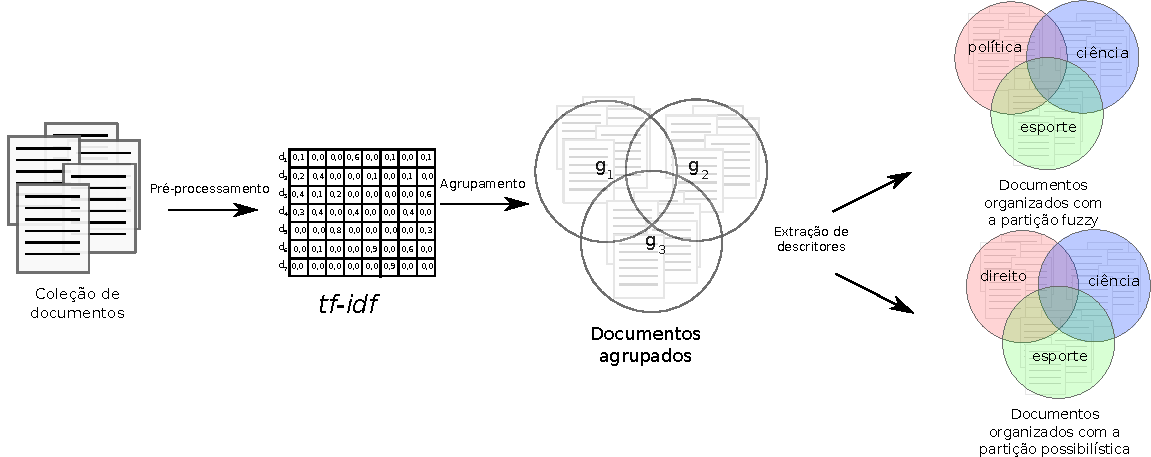
\includegraphics[width=1.0\columnwidth]{assets/process_pfcm.pdf} 
  \caption{Estratégia de organização flexível de documentos adotada ao se misturar abordagens fuzzy
  e possibilísticas no agrupamento} 
  \label{fig:flexibleorganization} 
\end{figure}

Para se calcular a quantidade ótima de grupos, para cada base de dados foi utilizado o
método da silhueta fuzzy (equação \ref{eq:fs}), método bastante utilizado com o propósito de avaliar
o agrupamento de documentos. Assim sendo, o número ideal de grupos é determinado após a execução da
silhueta fuzzy variando o número de grupos entre 2 e o número de classes de cada coleção.
Ressalta-se que em coleções que os dados não possuem rótulos, ou seja o número de classes é
desconhecido, ainda é possível usar o método da silhueta fuzzy para definir o número ótimo de
grupos. No entanto, a quantidade máxima de grupos deve ser definida de modo empírico ou com base em
alguma informação prévia a respeito dos dados. 

Para permitir uma análise comparativa dos resultados, o experimento foi realizado também com os
algoritmos FCM e PCM.
Como resultado do agrupamento das bases, está disposto na tabela \ref{table:pfcmclusters}, a
comparação do número de grupos obtidos no experimento. Nessa comparação nota-se que os algoritmos
FCM e PFCM foram os que alcançaram uma quantidade de partições mais próxima da quantidade de classes
existentes em cada coleção. Enquanto o PCM manteve uma tendência a produzir uma quantidade menor de
grupos em relação aos demais.

\begin{table}[!htp]
  \centering
  \begin{tabular}{ |l|c|c|c|c|}
    \hline
    {\bf Coleção} & {\bf \# classes} & {\bf FCM} & {\bf PCM} & {\bf PFCM} \\
    \hline
    Opinosis & 3 & 3 & 3 & 3 \\
    \hline
    20Newsgroup & 4 & 2 & 2 & 2 \\
    \hline
    Hitech & 6 & 6 & 5 & 5 \\
    \hline
    NSF & 16 & 11 & 2 & 16 \\
    \hline
    WAP & 20 & 14 & 5 & 16 \\
    \hline
    Reuters-21578 & 43 & 22 & 11 & 36 \\
    \hline
  \end{tabular}
  \caption{Quantidade ótima de grupos determinada através do método da silhueta fuzzy para cada
  algoritmo de agrupamento}
  \label{table:pfcmclusters}
\end{table}

Após agrupar os dados utilizando os métodos FCM, PCM e PFCM, foi aplicado o método de extração 
de descritores Soft-FDCL. Para nos permitir avaliar os descritores produzidos, foi verificado o
potencial preditivo dos mesmos, possibilitando assim quantificar a qualidade dos
termos selecionados para nomear os grupos. 

A avaliação do potencial preditivo dos descritores foi realizada, considerando cada grupo produzido
pelo pelo agrupamento como uma classe, ou seja, se durante o agrupamento foi gerado o conjunto de
grupos $G = \{g_1,g_2,...,g_c\}$, temos então o conjunto de classes $C =
\{classe_1,classe_2,...,classe_c\}$, onde cada $classe_i$ corresponde ao grupo $g_i$. No entanto, como as partições fuzzy e possibilística permitem 
que
um documento pertença a um ou mais grupos, foi considerado que a classe de um documento $d_i$,
como sendo a $classe_j$ do respectivo $grupo_j$, no qual $d_i$ possua a maior
pertinência/tipicidade. Esta definição está formalizada na equação \ref{eq:class}.
\begin{equation}
  classe(d_i) = \begin{cases}
    classe_j, & \mu(d_i,g_j) = \displaystyle\max_{\forall g \in G} \mu(d_i,g), \text{se a partição
  for fuzzy}\\
  classe_j, & \lambda(d_i,g_j) = \displaystyle\max_{\forall g \in G} \lambda(d_i,g), \text{se a
  partição for possibilística}
  \end{cases}
  \label{eq:class}
\end{equation}
Após atribuir as classes aos documentos, é produzida uma outra matriz,
considerando apenas os termos descritores dos grupos. Logo essa matriz documentos x descritores
$D'_{n \times m}$, 
é uma versão condensada da matriz documentos x termos $D_{n \times k}$, onde seja $n$ a 
quantidade de documentos, $k$ a quantidade de termos e $m$ a quantidade descritores. O conteúdo
dessa matriz condensada, assim como na matriz original, também é a frequência dos descritores nos 
documentos. 

Visando então avaliar a qualidade dos descritores e permitir uma comparação direta dos impactos
dessa abordagem com os resultados publicados em \citeonline{Nogueira2013} e
\citeonline{Nogueira2015}. Submeteu-se a matriz $D'$ 
aos algoritmos de classificação 
SVM, Naive Bayes, Multinomial Naive Bayes, KNN e C4.5, que são bem comuns na avaliação de 
métodos de aprendizado de máquina, e foram os mesmos utilizados em \citeonline{Nogueira2015}.

Nesse contexto, foi utilizado a implementação dos algoritmos de classificação citados anteriormente
, presentes na ferramenta WEKA\cite{weka}. Os algoritmos Naive Bayes (NB), Multinomial Naive Bayes
(NB-Multinomial) e o J48 (que é a implementação do C4.5 existente no WEKA), foram executados com os
parâmetros padrão da ferramenta. Por outro lado o SVM foi ajustado para usar o {\it Normalized
Polynomial Kernel\/} com o parâmetro de complexidade sendo $c = 2.0$. O algoritmo IBk (implementação
do KNN presente no WEKA) foi executado 7 vezes, variando o parâmetro de vizinhos de 1 até 7, sendo
escolhido o melhor resultado. Ressalta-se que foi adotada a técnica {\it 10-fold cross validation\/}
no experimento para melhor capturar a capacidade de generalização do modelo. O resultado dessa
classificação está apresentado nas figuras \ref{fig:pfcmopinosis},  \ref{fig:pfcm20news},
\ref{fig:pfcmhitech}, \ref{fig:pfcmnsf}, \ref{fig:pfcmwap} e \ref{fig:pfcmreuters}. 

\begin{figure}[!htp] \centering 
   \begin{minipage}{0.45\textwidth} 
     \centering
    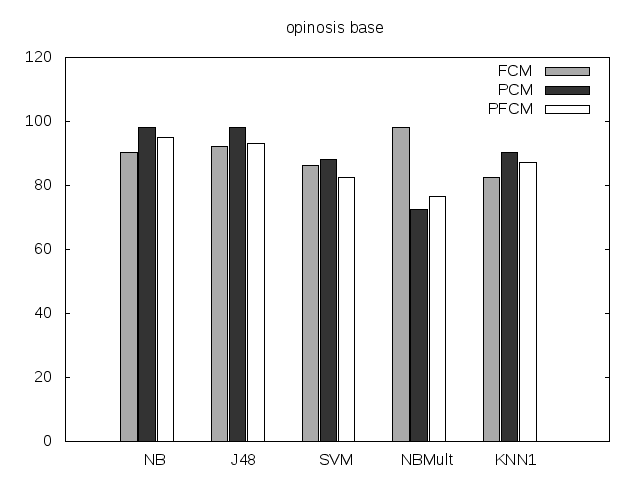
\includegraphics[width=1.0\columnwidth]{assets/pfcm/opinosis} 
    \caption{Desempenho obtido com os descritores extraídos com o algoritmo Soft-FDCL a partir dos
      métodos de agrupamento FCM,
    PCM e PFCM executados na coleção Opinosis} 
  \label{fig:pfcmopinosis}
  \end{minipage}\hfill 
  \begin{minipage}{0.45\textwidth} \centering
    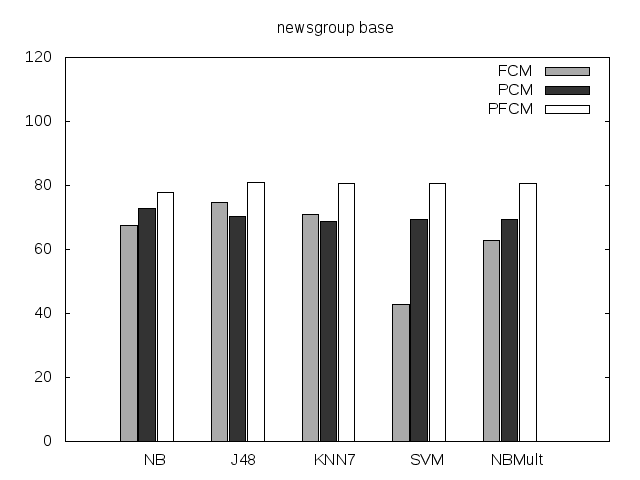
\includegraphics[width=1.0\columnwidth]{assets/pfcm/newsgroup} 
    \caption{Desempenho obtido com os descritores extraídos com o algoritmo Soft-FDCL a partir dos
      métodos de agrupamento FCM,
    PCM e PFCM executados na coleção 20Newsgroup} 
     \label{fig:pfcm20news} 
   \end{minipage} 
\end{figure}

\begin{figure}[!htp] \centering 
   \begin{minipage}{0.45\textwidth} 
     \centering
    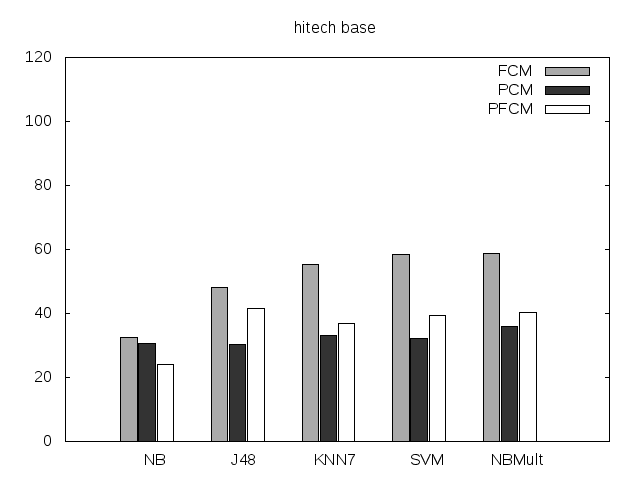
\includegraphics[width=1.0\columnwidth]{assets/pfcm/hitech} 
    \caption{Desempenho obtido com os descritores extraídos com o algoritmo Soft-FDCL a partir dos
      métodos de agrupamento FCM,
    PCM e PFCM executados na coleção Hitech} 
  \label{fig:pfcmhitech}
  \end{minipage}\hfill 
  \begin{minipage}{0.45\textwidth} \centering
    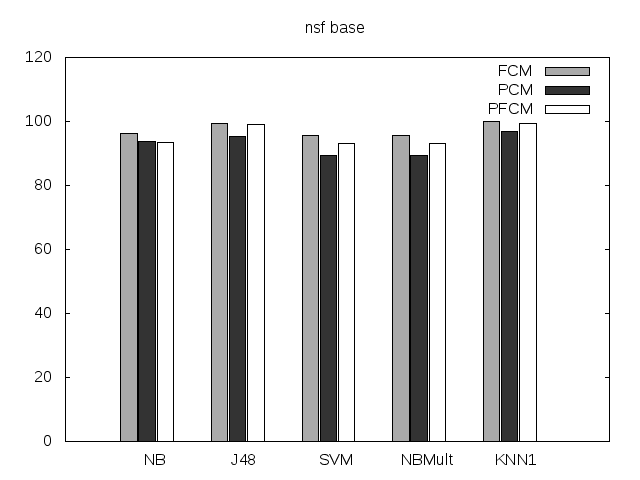
\includegraphics[width=1.0\columnwidth]{assets/pfcm/nsf} 
    \caption{Desempenho obtido com os descritores extraídos com o algoritmo Soft-FDCL a partir dos
      métodos de agrupamento FCM,
    PCM e PFCM executados na coleção NSF} 
     \label{fig:pfcmnsf} 
   \end{minipage} 
\end{figure}

\begin{figure}[!htp] \centering 
   \begin{minipage}{0.45\textwidth} 
     \centering
    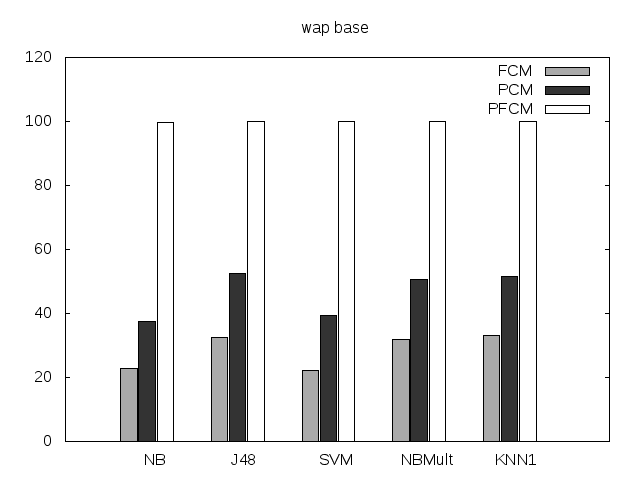
\includegraphics[width=1.0\columnwidth]{assets/pfcm/wap} 
    \caption{Desempenho obtido com os descritores extraídos com o algoritmo Soft-FDCL a partir dos
      métodos de agrupamento FCM,
    PCM e PFCM executados na coleção WAP} 
    \label{fig:pfcmwap}
  \end{minipage}\hfill 
  \begin{minipage}{0.45\textwidth} \centering
    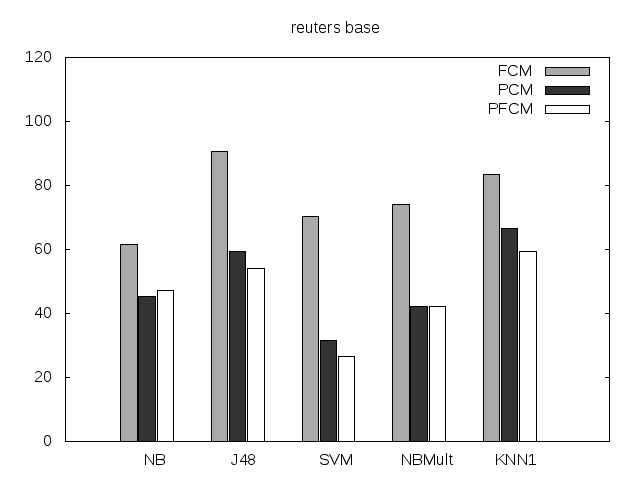
\includegraphics[width=1.0\columnwidth]{assets/pfcm/reuters} 
    \caption{Desempenho obtido com os descritores extraídos com o algoritmo Soft-FDCL a partir dos
      métodos de agrupamento FCM,
    PCM e PFCM executados na coleção Reuters-21578} 
     \label{fig:pfcmreuters} 
   \end{minipage} 
\end{figure}

O resumo dos resultados do desempenho dos descritores extraídos após o agrupamento com os
algoritmos FCM, PCM e PFCM é apresentado na Tabela \ref{table:pfcmsummary}. Na tabela, a marcação
($\checkmark$) denota qual método de agrupamento obteve a maior taxa de classificação dentre os
demais.

\begin{table}[!htp]
  \centering
  \begin{tabular}{ |l|c c c c c c c|}
    \hline
    {\bf nome} & docs & termos & classes & \% zeros & FCM & PCM & PFCM \\
    \hline
    {\bf Opinosis} & 51 & 842 & 3 & 95,73\% & & $\checkmark$ &  \\
    \hline
    {\bf 20newsgroups} & 2000 & 11028 & 4 & 99,11\% & & & $\checkmark$\\
    \hline
    {\bf Hitech} & 600 & 6925 & 6 & 97,93\% & $\checkmark$ & & \\
    \hline
    {\bf NSF} & 1600 & 2806 & 16 & 99,76\% & $\checkmark$ & & \\
    \hline
    {\bf WAP} & 1560 & 8070 & 20 & 98,51\% & & & $\checkmark$ \\
    \hline
    {\bf Reuters-21578} & 1052 & 3925 & 43 & 98,55\% & $\checkmark$ & & \\
    \hline
  \end{tabular}
  \caption{Sumário dos resultados da classificação dos descritores}
  \label{table:pfcmsummary}
\end{table}

Esses resultados obtidos reforçam a flexibilidade e adaptação do método Soft-FDCL
\cite{Nogueira2013}, a novos algoritmos de agrupamento. De modo que o método se demonstra promissor
na tarefa extrair termos relevantes dos grupos produzidos na etapa de agrupamento, e isso é
demonstrado através do potencial preditivo evidenciado na Tabela \ref{table:pfcmsummary}, com as
taxas máximas de classificação de mais de 80\% para quase todas as bases, com exceção da base
Hitech, a qual obteve a taxa máxima de 58.67\%.  Por outro lado, ressalta-se a importância também de
avaliar de maneira subjetiva os descritores selecionados dos grupos, pois isso nos permite
compreender melhor se os termos obtidos fazem sentido. 

\begin{table}[!htp]
  \centering
  \begin{tabular}{ |l|p{4cm} | p{4cm} | p{4cm}|}
    \hline
    {\bf método} & $classe_1$ & $classe_2$ & $classe_3$ \\
    \hline
    {\bf FCM} & easy, clear, drive, display, control, car, version, nice, work, perfect & fact,
    import, isn't, model, problem, unit, design, don't, doesn't, found & breakfast, nearby,
    concierge, eat, bottle, coffee, floor, food, inn, friendly \\
    \hline
    {\bf PCM} & easy, read, problem, version, don't, small, nice, car, work, found & fact, back,
    turn, expect, size, close, quality, review, min, feature & feel, amazing, isn't, extreme, drive,
    include, point, reason, give, run\\
    \hline
    {\bf PFCM $\mu$} & easy, drive, control, don't, version, nice, car, work, perfect, lot & fact,
    isn't, read, complete, device, display, size, doesn't, found & breakfast, nearby, pleasant,
    concierge, eat, coffee, floor, clean, friendly, food\\
    \hline
    {\bf PFCM $\lambda$} & club, immaculate, send, towel, basic, exception, spotl, pillow, typical,
    fridge & pub, housekeep, holiday, tourist, tea, smoke, pm, renovate, facilite, london & usual,
    central, forum, bottle, modern, adult, supply, food, reserve, dinner\\
    \hline
  \end{tabular}
  \caption{Descritores extraídos com os métodos de agrupamento FCM, PCM e PFCM da coleção Opinosis,
  onde $\mu$ e $\lambda$ se referem as partições fuzzy e possibilística respectivamente, da qual os
descritores foram extraídos.}
  \label{table:pfcmdescriptors}
\end{table}

Para realizarmos uma análise subjetiva dos resultados, foi escolhido os descritores obtidos da base
de dados Opinosis, por possuir poucos grupos e assim facilitar a análise e a visualização. A coleção
Opinosis contém opiniões dos usuários a respeito de serviços de hospedagem, dispositivos eletrônicos
e carros.  Portanto na Tabela \ref{table:pfcmdescriptors} temos a seleção de termos descritores
escolhidos para cada grupo, pelos respectivos métodos de agrupamento. Ao analisarmos os termos
selecionados é possível notar uma tendência geral, da $classe_1$ conter palavras relacionadas a
carros, a $classe_2$ abordando opiniões dos usuários sobre dispositivos eletrônicos e a $classe_3$
com opiniões a respeito dos serviços de hospedagem e alimentação. Contudo nota-se que os descritores
do PCM e do PFCM$\lambda$ (descritores da partição possibilística do PFCM) estão um pouco mais
misturados, não apresentando uma tendência geral bem definida. Uma explicação possível a esse
resultado, pode se encontrar na própria partição possibilística a qual permite que um mesmo
documento possua um grau de tipicidade elevado em todos os grupos. Portanto uma solução possível,
pode ser uma adaptação do método de extração de descritores Soft-FDCL voltado para a partição
possibilística, assim como também para algoritmos híbridos com duas partições, que é o caso do PFCM.

De maneira complementar, é importante salientar que o método de extração de descritores Soft-FDCL é
totalmente influenciado pelos valores contidos nas partições fuzzy e possibilística. Portanto, é
também importante se realizar uma análise dos métodos de agrupamento utilizados no experimento, com
a finalidade de se entender qual método é mais apropriado em determinados contextos. Nesse contexto
os resultados apontam que a dimensionalidade das bases foi um fator determinante no desempenho dos
métodos de agrupamento no contexto da organização flexível de documentos, e consequentemente a
extração de descritores. Por exemplo, do sumário de resultados apresentados na Tabela
\ref{table:pfcmsummary}, podemos observar que a o método PCM obteve o melhor resultado na coleção
Opinosis, que possui a menor dimensionalidade (842 termos), enquanto que o algoritmo FCM superou os
demais métodos nas bases NSF (2806 termos), Reuters-21578 (3925 termos), Hitech (6925 termos), e por
fim o algoritmo PFCM atingiu melhores resultados para as bases WAP (8070 termos) e 20Newsgroup
(11028 termos), que são as bases de maior dimensionalidade na coleção.

Na próxima sessão, motivado pelos resultados desse experimento será explorado uma adaptação do
método Soft-FDCL para evitar o processo de extração dupla de descritores em algoritmos que possuam
partições fuzzy e possibilística.

\section{Método Mixed-PDCL}

No experimento anterior identificamos um possível problema ao realizar a extração dos
descritores de maneira separada em cada partição do PFCM, assim como também foi apontado que o
método pode não capturar toda essência da partição possibilística, que difere da partição fuzzy do
FCM por não possuir a restrição que obriga a soma das pertinências de um grupo ser igual a um
(equação \ref{eq:fcmrestri1}).
Logo, é intuitivo indagar, que para uma melhor interpretação dos grupos produzidos em um método de
agrupamento híbrido, seja pertinente utilizar também uma abordagem mista de extração descritores.
Aproveitando-se assim dos benefícios existentes na partição possibilística, a qual penaliza os
elementos ruidosos, com baixos valores de tipicidade, sem abrir mão das vantagens presentes na
partição fuzzy. Para isso é necessário se compreender os mecanismos de funcionamento do método
Soft-FDCL, para que seja possível propor uma adaptação para este contexto.

O método Soft-FDCL ({\it Soft Organization - weighted Fuzzy Description Comes Last}) proposto em 
\citeonline{Nogueira2013}, é baseado em uma adaptação das medidas clássicas de Recuperação de
Informação (RI), para quantificar a relevância dos termos candidatos a descritores dos grupos
obtidos na etapa de agrupamento, utilizando a informação de pertinência ou tipicidade advinda do
algoritmo de agrupamento.  Esse grau de compatibilidade entre o documento e o grupo, desempenha um
papel fundamental na seleção dos termos candidatos a descritores de um determinado grupo, pois
através deste, é possível penalizar os termos de documentos que possuam baixo grau de
compatibilidade com grupo o qual o descritor está sendo extraído.  

Para realizar a extração dos descritores, inicialmente todos os termos que permanecem na coleção
após a etapa de pré-processamento são considerados como candidatos a descritores. Posteriormente o
método realiza uma avaliação quantitativa da relevância de cada termo $t_k$ para um grupo $g_j$,
utilizando a medida $f1$ apresentada na equação \ref{eq:fmeasure}, que é a média harmônica da
precisão (equação \ref{eq:precision}) e da revocação (equação \ref{eq:recall}).
A medida de precisão checa a quantidade de documentos significantes entre os documentos
recuperados. Enquanto a medida de revocação calcula a proporção de documentos relevantes recuperados
entre todos os documentos relevantes da coleção. Tanto a medida de precisão e de revocação, tomam
como base as informações obtidas a partir da matriz de contingência apresentada na Tabela
\ref{table:softmatrix}. Adicionalmente tem-se que um documento $d_i$ é considerado como parte do
grupo $g_j$, caso $\mu(d_j,g_j) \geq \delta$ para valores de pertinências ou $\lambda(d_i,g_j) \geq
\delta$ para partição possibilística, onde seja $\delta = \frac{1}{c}$ e $c$ a quantidade de
grupos. O limiar $\delta$ é uma parte relevante do método Soft-FDCL, pois ele possibilita se
considerar como candidatos a descritores, os termos presentes em documentos que pertençam a mais de
um grupo, ao mesmo tempo que também penaliza os termos presentes em documentos com baixa
compatibilidade em um grupo.

Portanto, para efetuar a seleção dos termos descritores, é construído um $ranking$ dos termos
candidatos de cada grupo, ordenados pela pontuação obtida com a medida $f1$ (equação
\ref{eq:fmeasure}). A partir dessa pontuação, é selecionado os termos com as maiores
pontuações em cada grupo. \citeonline{Nogueira2013} destaca, que a quantidade de descritores a ser
selecionada fica a critério do usuário.

\begin{table}[!htp]
  \centering
  \begin{tabular}{ |p{5cm}|p{5cm}|p{5cm}|}
    \cline{2-3}
    \multicolumn{1}{p{5cm}|}{} & Documentos do grupo $g_j$ com grau de compatibilidade 
    maior ou igual a $\delta$ &
    Documentos do grupo $g_j$ com grau de compatibilidade menor do que $\delta$ \\
    \hline
    Documentos que possuem o descritor candidato $t_k$ & \parbox[c]{5cm}{\centering $ganhos$} &
    \parbox[c]{5cm}{\centering \it ruídos\/} \\
    \hline
    Documentos que não possuem o descritor candidato $t_k$ & \parbox[c]{5cm}{\centering $perdas$} &
    \parbox[c]{5cm}{\centering $rejeitos$} \\
    \hline
  \end{tabular}
  \caption{Matriz de contingência do termo $t_k$ para o grupo $g_j$ para as medidas de recuperação
  de informação}
  \label{table:softmatrix}
\end{table}

\begin{equation}
  precis\tilde{a}o(t_k,g_j) = \frac{ganhos}{ganhos + \text{\it ruídos}}
  \label{eq:precision}
\end{equation}
\begin{equation}
  \text{\it recuperação\/}(t_k,g_j) = \frac{ganhos}{ganhos + perdas}
  \label{eq:recall}
\end{equation}
\begin{equation}
  f1(t_k,g_j) = \frac{2 * \text{\it precisão}(t_k,g_j) * \text{\it recuperação}(t_k,g_j)}
  {\text{\it precisão}(t_k,g_j) + \text{\it recuperação}(t_k,g_j)}
  \label{eq:fmeasure}
\end{equation}

Em síntese o método SoftO-FDCL, cria uma tabela de pontuação dos termos candidatos aos grupos,
e seleciona os que obtiverem a maior quantidade de pontos. Bem como a promoção a termo candidato é
feita considerando os termos que ocorrem em documentos com grau de compatibilidade maior que o
limiar $\delta = \frac{1}{c}$. Ao se considerar esse limiar em em partições com graus de
pertinência, como a partição fuzzy do FCM, esse limiar $\delta$ se mostra adequado, pois como foi
definido no capitulo 2, o grau de compatibilidade do FCM é restrito a equação \ref{eq:fcmrestri1}.
Portanto ao filtrar os documentos em uma partição de pertinências utilizando $\delta$ como critério
de corte, na maioria das vezes será descartado algum documento no processo. 

Formalizando essa
percepção, podemos então definir as duas propriedades  que derivam dessa discussão, as quais são as
equações (\ref{eq:limiarp1}) e (\ref{eq:limiarp2}), onde seja $c$ a quantidade de grupos. A primeira
propriedade (equação \ref{eq:limiarp1}) expressa que se um documento possuir pertinência maior do
que o limiar $\delta$ em um grupo $g_1$ qualquer, obrigatoriamente existirá ao menos um outro grupo
$g_2$ no qual esse mesmo documento terá pertinência inferior ao limiar $\delta$. Portanto, essa
propriedade nos indica que na maioria das vezes um ou mais documentos serão descartados na análise
dos termos candidatos do grupo, o que reforça a adequação desse limiar para a partição de
pertinências. Por outro lado, a segunda
propriedade (equação \ref{eq:limiarp2}) denota o único caso particular, no qual um documento $d_i$
não será descartado em nenhum grupo. Isto ocorre apenas se $d_i$ possuir pertinência igual em todos
os grupos, o que só acontece em dados ruidosos, que apresentam o problema do elemento equidistante
detalhado na Figura \ref{fig:fcm_problem} do capítulo 2.

\begin{equation}
  \mu(d_1,g_j) > \delta \rightarrow \exists \mu(d_i, g_2) < \delta
  \label{eq:limiarp1}
\end{equation}
\begin{equation}
  ( \mu(d_1,g_1) = \delta ) \wedge ( \mu(d_i,g_2) = \delta ) \wedge ... \wedge ( \mu(d_i,g_{c_1}) =
  \delta ) \rightarrow ( \mu(d_i, g_c) = \delta  )
  \label{eq:limiarp2}
\end{equation}

Contudo, para a partição possibilística, essas duas propriedades não são satisfeitas. Isso se deve,
por conta da remoção da restrição da equação (\ref{eq:fcmrestri1}), o que possibilita que
o grau de compatibilidade da partição possibilística variar de maneira independente entre o intervalo
de $[0,1]$ sem ser influenciado pelo grau de compatibilidade do documento nos demais grupos.





\section{Método HPCM}
\section{Considerações finais}
